Within recent years numerous research papers have emerged showing successful applications of various methods to real word problems like detecting faults, benchmarking, classifying, predicting or recognizing patterns in the energy consumption of buildings. Most of the applied methods rely on theories rooted in the fields of statistics, machine learning and data mining to analyze and interpret the data. To successfully apply such methods to real word problems one must be familiar with the nature of the data, and have working knowledge of the methods being applied. This section will explore some of these methods and the current literature that applies them to various problems related to energy management.

\section{Decomposing time series}
The most visible pattern that emerge from time series data of building energy consumption is the daily rise and fall in consumption, which loops every 24 hours following the daily cycles of building users. Also a weekly cycle can be noticed, as different days of the week tend to have different consumption profiles. If looking at several years of data, the yearly cycle following the seasonal changes in environmental conditions can be seen. These cycles form the basis for the components that can be found when decomposing a time serie, and which could be used to reconstruct the original by combining the components. For instance considering the weekly cycles and yearly seasonal change, it would be possible to make a decomposition into a Cyclical Component, and a Seasonal Component\footnote{http://en.wikipedia.org/wiki/Decomposition\_of\_time\_series}. Additionally suggests that the decomposition produces a Trend Component  and an Irregular Component. The Trend Component reflects the long term progression irrespective of any cycles and seasonality, while the Irregular Component is the noise in the original time serie which could not be explained with the other components. Figure 4.1 shows an example of a decomposition.
\begin{figure}
\begin{center}
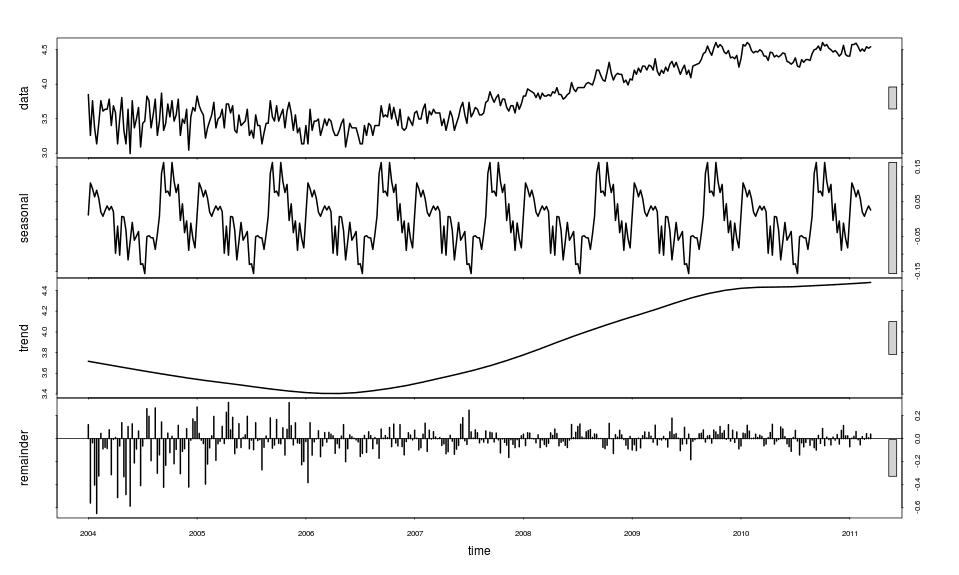
\includegraphics[scale=0.2]{stldecomposition.jpg}
\end{center}
\caption{Decomposition of time series}
\end{figure}
\newline
\newline
The example illustrates how decomposing time series of energy consumption can give more insight into the nature of the consumption. We can see that the consumption is generally going up each year, and that consumption is higher in the winter than in the summer. Decomposition is relevant when comparing consumption between different days, because it might be beneficial to first remove the seasonality component. There are however many ways to adjust for seasonality. For instance \cite{faultdetec2} suggests subtracting from each day the minimum consumption for that day, while \cite{faultdetec4} transforms the features of one day by determining the difference
between it and a the features of a 1-week average of surrounding days. 

The different components of a decomposition can serve as different units of analysis, and are therefore important to consider when extracting features from the data. Whatever forecasting consumption load, detecting abnormal consumption or something else is desired, most approaches agree upon that the first step is to extract interesting features from the data, which can be used in an analysis. This might be raw consumption figures (daily average, daily max/min), ratios between features (consumption night/day), temporal properties (time of daily max, first time above 1kW) or statistical properties (variance, correlation between features). \cite{Benchmarking1} brings a list of potentially interesting features when considering energy consumption data, while \cite{Benchmarking2} suggests a range of interesting building properties to consider. 
\section{Cluster analysis}
Cluster analysis is widely used within data mining and machine learning, to find underlying structures and patterns in data. \cite{faultdetec4} proposes a pattern recognition algorithm for determining days of the week based on the raw consumption data, and explains how this information can be used for both forecasting consumption load and detecting abnormal consumption. By creating a cluster for each day of the week and then identifying similar clusters based on various features of daily consumptions, it is possible to come up with a number of ‘day types’ with distinct consumption profiles. The type of day and consumption profile can then be used as input to forecasting algorithms, or as a model of normal consumption from which a large deviation can be considered an anomaly. \cite{faultdetec2} uses a very similar approach.

There are many different techniques for clustering, and even more algorithms implementing them. Some popular ones are the the centroid-based K-means algorithm and the density- based DBSCAN. The K-means algorithm fixes the number of clusters to k (a parameter given to the algorithm). The algorithm will assign each data point in the dataset to the nearest cluster center, and then seek to find the optimal positions for the k cluster centers, such that the squared distances from each object to the cluster centers is minimal. K-medoids clustering is very similar to k-means, except that while the cluster is represented by a centroid in k-means, it is represented by the data point closest to the center of the cluster in k-medoids. A drawback of this approach is that K-means and K-medoids clustering does not work well with non convex clusters, which might be present if data point features do not follow normal distributions. This problem is avoided in DBSCAN which creates clusters by connecting points which have a specified minimum number of other points within a specified radius. Based on this density criterion clusters will of following arbitrary shapes can be formed. Figure 4,2 illustrates how cluster analysis with K-means and DBSCAN can result in very different clusters for the same dataset.
\begin{figure}
\begin{center}
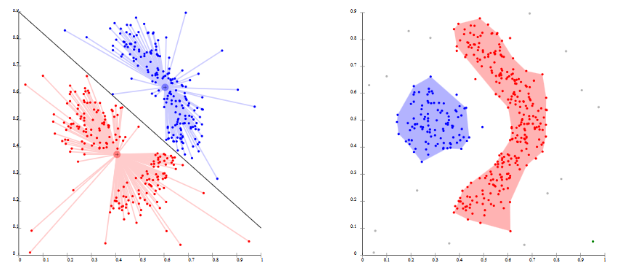
\includegraphics[scale=0.5]{cluster.png}
\end{center}
\caption{\emph{Note these pictures have been taken from Wiki -Cluster analysis}}
\end{figure}
DBSCAN additionally has the ability to detect outliers, which would be the data points residing in low density areas not reachable with the density criterion. \cite{faultdetec3} compares the use of DBSCAN alone with using K-means followed by the Generalized Extreme Studentized Deviate (GESD) outlier detection method, to find  outliers and detect faults in building energy consumption. The results however seem somewhat inconclusive. 
\newline

\cite{Benchmarking1} and \cite{Benchmarking2} demonstrates the use of SOMs (Self Organizing Maps) to perform cluster analysis of building energy consumers. \cite{Benchmarking1} finds clusters of energy consumers by training a SOM using raw energy consumption data, while \cite{Benchmarking2} uses building information as basis for the clustering.
Perhaps as important as the clustering method is the features chosen to use as input for the clustering. Too many features might introduce too much noise, so it might be beneficial with some dimensionality reduction before performing cluster analysis. Using too few features however might not properly separate the clusters. A dimensionality reduction can be achieved with a principal component analysis. By using only the principal components that explain the majority of variation, one would have found the best low-dimensional representation of the variation in a multivariate data set. \cite{faultdetec2} argues that a better approach to use when classification is the purpose is CVA (canonical variate analysis), known as linear discriminant analysis (LDA). The purpose of LDA is to find the linear combinations of the original variables that gives the best possible separation between the groups. Thus LDA is used with day of week as the grouping variable, to project the original data into new axes which maximize separation between different days\footnote{A more in depth explanation of PCA and LDA can be found in: http://little-book-of-r-for-multivariate-analysis.readthedocs.org/en/latest/src/multivariateanalysis.html}.
\section{Detecting faults}
Detecting abnormal energy consumption seems always to follow the basic steps of building some kind of model of normal consumption and then detecting faults with an appropriate outlier detection method \cite{faultdetec1}, \cite{faultdetec2} and \cite{faultdetec3}. Another approach would be to use supervised learning to train a classifier that can distinguish faulty consumption from normal. However this would require a proper training set with already identified and labeled errors for each building. The lack of such datasets and the fact that faulty consumption is a fairly rare event, makes the outlier detection approach the favoured one. Apart from using outlier detection methods to detect abnormal consumption, it is used as a preprocessing method to remove data points which are so unusual that they could indicate a measurement error.

An outlier can be defined as data which appear to be inconsistent with the rest of the data set, like for instance a numerical value which is significantly distant from the rest of the data set. There is no mathematically rigid method for defining an observation as an outlier, and many methods to detect outliers both in univariate and multivariate data sets have been proposed. If the data is approximately normally distributed univariate outliers can easily be identified with a hypothesis test calculating the p-value which is the probability obtaining a result equal to or more extreme than what was actually observed. \cite{faultdetec2}, \cite{faultdetec3} and \cite{faultdetec4} all make use of the GESD generalized extreme studentized deviate [REF måske?] univariate outlier detection method. This method works by doing Grubbs’ test which is defined for the hypothesis:
\newline

$H_0$: There are no outliers in the data set
\newline

$H_A$: There is at least one outlier in the data set 
\newline
\newline
If there is an outlier it is removed and the test is performed again, until a specified upper limit is reached or there are no more outliers in the data set. Besides an upper limit on the number of outliers an significance level $\alpha$ must be specified which would translate into the probability of getting a false positive. 

In \cite{faultdetec2} the GESD procedure is applied to each feature of an observation to detect an outlier. However as figure 4,3 illustrates, an outlier in a multidimensional dataset is not always an univariate outlier. Considering the $x$ and $y$ values independently does not obviously reveal the outlier flagged in the first graph. 
\begin{figure}
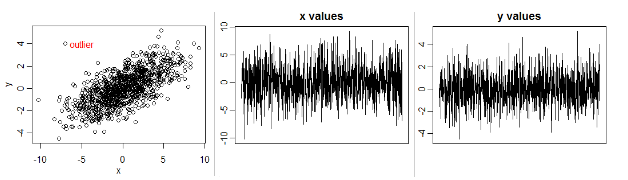
\includegraphics[scale=0.75]{outlier.png}
\caption{Multivariate outliers}
\end{figure}
To deal with multivariate outliers one needs a proper method capable of considering the correlation between variables when detecting them. One such method is PCOut \cite{OutDetec1}. PCOut is an advanced algorithm which utilize inherent properties of principal components decomposition for outlier detection in high dimensional data. It does not require that the data come from any particular distribution, and is computationally fast.
